\section{INTRODUCTION AND MOTIVATION}
\label{sec:intro}

Protons and neutrons make up almost all of the visible mass in the universe, yet their internal structure is still only partly understood. We know the theory that governs them. Quantum Chromodynamics (QCD) describes quarks and gluons interacting through the exchange of color charge, and its Lagrangian fits on a single line. What we cannot do in general is solve it. At the distance scale of a nucleon, about one femtometer, the QCD coupling is large, perturbation theory does not converge, and the quarks and gluons are permanently confined inside hadrons. The properties of the nucleon therefore have to be extracted from experiment through well-defined observables or computed numerically from first principles.

This thesis is about one such observable, the Sivers function $f_{1T}^\perp$. It describes how the transverse momentum of an unpolarized quark is correlated with the transverse spin of the nucleon that contains it. We compute the Sivers function with lattice QCD and, unlike earlier lattice calculations, we resolve its dependence on the longitudinal momentum fraction $x$ carried by the quark. This chapter explains where the Sivers function comes from, why it matters, what experiments have measured, and what a lattice calculation can add. It closes with a summary of the contributions of this work and an outline of the remaining chapters.

\subsection{From form factors to partons}
\label{sec:intro_partons}

The first direct evidence that the proton has a finite size came from elastic electron scattering. In the 1950s Hofstadter and collaborators measured the angular distribution of electrons scattered off hydrogen and found that it fell below the prediction for a point charge. The deviation is described by form factors, which are Fourier transforms of the charge and magnetization distributions, and it corresponds to a proton radius of roughly $0.8$~fm \cite{Hofstadter:1956qs}.

A decade later, the SLAC-MIT experiments pushed the electron energy high enough to break the proton apart. In this deep inelastic scattering (DIS) regime the cross section showed a surprising feature: at large momentum transfer $Q^2$ it depended, to a good approximation, only on the dimensionless ratio $x_B = Q^2/(2P\cdot q)$ and not on $Q^2$ separately \cite{Bloom:1969kc,Breidenbach:1969kd}. Bjorken had predicted this scaling behavior from current algebra \cite{Bjorken:1968dy}. Feynman gave it a simple physical meaning \cite{Feynman:1969ej}: in a frame where the proton moves very fast, the virtual photon scatters incoherently off pointlike constituents, the partons, and $x_B$ is the fraction of the proton momentum carried by the struck parton. The observed relation between the two DIS structure functions, $F_2 = 2x F_1$, showed that the charged partons have spin $1/2$ \cite{Callan:1969uq}. They were identified with the quarks that Gell-Mann and Zweig had introduced to organize the hadron spectrum \cite{Gell-Mann:1964ewy,Zweig:1964jf}.

The parton picture raised a puzzle. If quarks are bound so tightly that no free quark has ever been observed, why do they behave as nearly free particles when struck hard? The answer came with non-Abelian gauge theory. Quarks carry a threefold color charge, and the color interaction is mediated by eight gluons that are themselves charged \cite{Yang:1954ek,Fritzsch:1973pi}. Gross and Wilczek \cite{Gross:1973id} and Politzer \cite{Politzer:1973fx} showed that in such a theory the effective coupling decreases logarithmically at short distances. This property, asymptotic freedom, explains Bjorken scaling and its slow logarithmic violation. The same running makes the coupling grow at long distances, which is consistent with confinement. QCD therefore describes both regimes, and the strong coupling at long distances is the reason nucleon structure has to be studied with non-perturbative tools.

\subsection{Beyond one dimension}
\label{sec:intro_3d}

The central objects of the parton model are the parton distribution functions (PDFs). The unpolarized quark PDF $f_1^q(x)$ gives the number density of quarks of flavor $q$ carrying momentum fraction $x$ in a fast-moving nucleon. PDFs are universal: the same functions describe DIS, the Drell-Yan production of lepton pairs in hadron collisions \cite{Drell:1970wh}, jet production at the LHC, and many other processes. This universality rests on collinear factorization theorems, which separate a hard partonic cross section, calculable in perturbation theory, from the non-perturbative distributions. PDFs have been determined from global fits to experimental data with high precision over a wide range of $x$.

A PDF, however, is a one-dimensional picture. It integrates over all the transverse degrees of freedom of the parton, both its position and its momentum in the plane perpendicular to the nucleon's direction of motion. Two extensions restore this information. Generalized parton distributions (GPDs), which appear in exclusive processes such as deeply virtual Compton scattering, encode the correlation between $x$ and the transverse position $\vprp{b}$ of the parton \cite{Muller:1994ses,Radyushkin:1997ki,Ji:1996ek,Diehl:2003ny}. At zero skewness, their Fourier transform in the momentum transfer gives impact-parameter distributions, which have a density interpretation \cite{Burkardt:2000za}. Transverse momentum dependent parton distributions (TMDs) instead describe the joint distribution in $x$ and the intrinsic transverse momentum $\vprp{k}$ \cite{Collins:1981uw,Mulders:1995dh,CollinsBook2011}. They appear in processes where a transverse momentum is measured that is small compared to the hard scale, such as semi-inclusive DIS (SIDIS) and Drell-Yan production at low transverse momentum of the lepton pair.

The idea that partons move transversely inside the nucleon is almost as old as the parton model. Cahn showed that intrinsic transverse momentum produces a $\cos\phi_h$ modulation of the SIDIS cross section \cite{Cahn:1978se}. Collins and Soper formulated the factorization of processes sensitive to transverse momentum \cite{Collins:1981uk,Collins:1981uw}, and Collins, Soper and Sterman used it to resum large logarithms in the transverse momentum distribution of Drell-Yan pairs \cite{Collins:1984kg}. The complete set of TMDs at leading power was classified for Drell-Yan by Ralston and Soper \cite{Ralston:1979ys} and for SIDIS by Kotzinian \cite{Kotzinian:1994dv} and by Mulders and Tangerman \cite{Tangerman:1994eh,Mulders:1995dh}. Their operator definitions, including the treatment of gauge links and rapidity divergences, reached their current form much later \cite{Ji:2004wu,CollinsBook2011,Aybat:2011zv}.

Both GPDs and TMDs can be obtained from a common parent, the generalized TMDs (GTMDs), whose Fourier transforms are quantum phase-space (Wigner) distributions in $x$, $\vprp{b}$ and $\vprp{k}$ \cite{Belitsky:2003nz,Meissner:2009ww,Lorce:2011kd}. Figure~\ref{fig:intro_hierarchy} sketches these relations. Together, GPDs and TMDs make up the program of nucleon ``tomography'', a central goal of the Electron-Ion Collider (EIC) now under construction \cite{Boer:2011fh,Accardi:2012qut,AbdulKhalek:2021gbh}.

\begin{figure}[htpb]
\centering
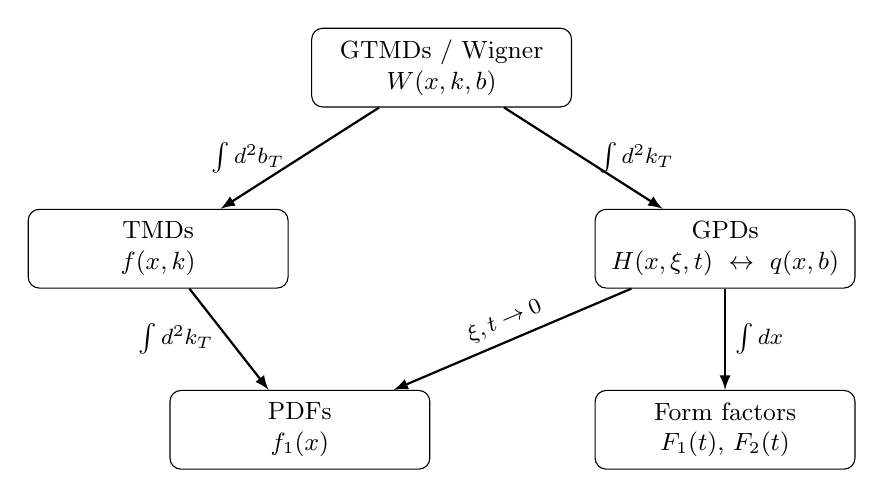
\begin{tikzpicture}[
    box/.style={draw, rounded corners, align=center, minimum width=3.3cm, minimum height=1.0cm, font=\small},
    arr/.style={-latex, thick}]
  \node[box] (gtmd) at (0,0) {GTMDs / Wigner\\ $W(x,\vprp{k},\vprp{b})$};
  \node[box] (tmd) at (-3.6,-2.3) {TMDs\\ $f(x,\vprp{k})$};
  \node[box] (gpd) at (3.6,-2.3) {GPDs\\ $H(x,\xi,t)\ \leftrightarrow\ q(x,\vprp{b})$};
  \node[box] (pdf) at (-1.8,-4.6) {PDFs\\ $f_1(x)$};
  \node[box] (ff) at (3.6,-4.6) {Form factors\\ $F_1(t),\,F_2(t)$};
  \draw[arr] (gtmd) -- node[left, font=\footnotesize, xshift=-2pt] {$\int d^2 b_T$} (tmd);
  \draw[arr] (gtmd) -- node[right, font=\footnotesize, xshift=2pt] {$\int d^2 k_T$} (gpd);
  \draw[arr] (tmd) -- node[left, font=\footnotesize, xshift=-2pt] {$\int d^2 k_T$} (pdf);
  \draw[arr] (gpd) -- node[above, font=\footnotesize, sloped] {$\xi,t\to 0$} (pdf);
  \draw[arr] (gpd) -- node[right, font=\footnotesize] {$\int dx$} (ff);
\end{tikzpicture}
\caption{Relations between the distributions that describe the quark structure of the nucleon. Integrating the generalized TMDs (or their Fourier transforms, the Wigner distributions) over transverse position gives TMDs, and integrating over transverse momentum gives GPDs. The collinear PDFs are obtained from TMDs by integrating over $\vprp{k}$ and from GPDs in the forward limit. Moments of GPDs in $x$ give the elastic form factors.}
\label{fig:intro_hierarchy}
\end{figure}

\subsection{Spin and single-spin asymmetries}
\label{sec:intro_ssa}

Spin measurements have repeatedly shown that this picture is incomplete. In 1988 the European Muon Collaboration measured the polarized structure function $g_1$ of the proton and concluded that the quark spins account for only a small fraction of the proton spin \cite{EuropeanMuon:1987isl}. The result, the ``proton spin crisis'', started a long program to understand how the spin of the nucleon is shared among quark spin, gluon spin, and orbital angular momentum \cite{Jaffe:1989jz,Ji:1996ek,Leader:2013jra}. Orbital motion requires transverse momentum, so TMDs are one natural place to look for it.

A second puzzle came from hadron collisions with a transversely polarized beam or target. Large transverse polarizations of $\Lambda$ hyperons produced in unpolarized proton collisions were observed in the 1970s \cite{Bunce:1976yb}, and large left-right asymmetries in the production of pions off transversely polarized protons were measured by the E704 experiment at Fermilab \cite{FNAL-E704:1991ovg}. Such transverse single-spin asymmetries (SSAs) were not expected. In collinear perturbative QCD, Kane, Pumplin and Repko showed that they are suppressed by the quark mass over the hard scale and by a power of $\alpha_s$ \cite{Kane:1978nd}, which makes them far too small to explain the data.

In 1990 Sivers proposed a mechanism beyond the collinear framework \cite{Sivers:1989cc}. If the transverse momentum distribution of quarks in a transversely polarized proton is not symmetric, but shifted in a direction perpendicular to the spin, then the produced hadrons inherit a preferred side, and a left-right asymmetry follows. The size of this effect is set by a new distribution function, today called the Sivers function $f_{1T}^\perp(x,\vprp{k}^2)$. For a nucleon moving along the $z$ direction with transverse spin $\vprp{S}$, the number density of unpolarized quarks reads
\begin{equation}
  f_{q/N^\uparrow}(x,\vprp{k}) = f_1^q(x,\vprp{k}^2) - \frac{\epsilon_{ij}\,k_{T,i}\,S_{T,j}}{\mN}\, f_{1T}^{\perp q}(x,\vprp{k}^2) \ ,
  \label{eq:intro_sivers_density}
\end{equation}
with $\epsilon_{12}=+1$, so that $\epsilon_{ij}k_{T,i}S_{T,j} = (\hat{\vect{z}}\times\vprp{k})\cdot\vprp{S}$. This is the ``Trento'' convention \cite{Bacchetta:2004jz}, and it is the form used throughout this thesis (compare Eq.~\eqref{eq-phigammaplus}). Figure~\ref{fig:intro_sivers_cartoon} illustrates the resulting distortion of the quark distribution in transverse momentum space.

\begin{figure}[htpb]
\centering
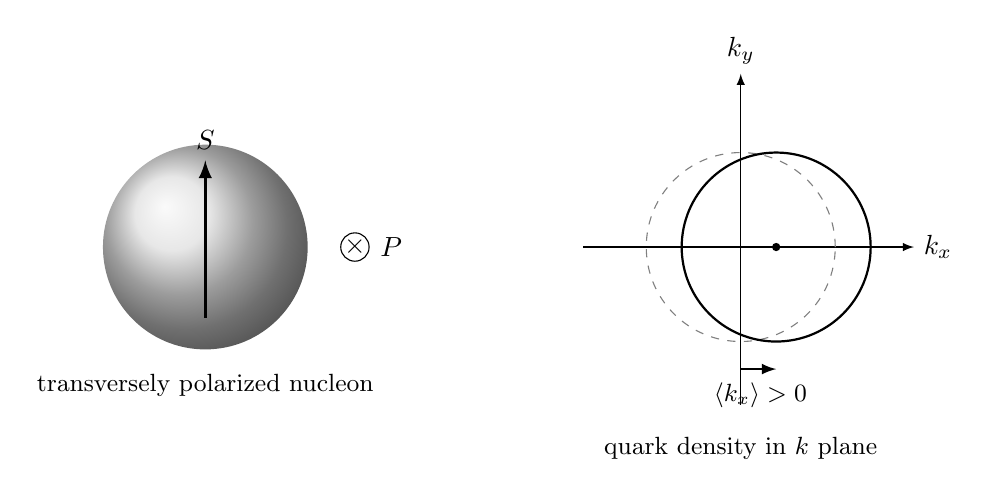
\begin{tikzpicture}[scale=1.0]
  % left panel: nucleon
  \begin{scope}[shift={(-4.2,0)}]
    \shade[ball color=gray!25] (0,0) circle (1.3);
    \draw[very thick, -latex] (0,-0.9) -- (0,1.1) node[above] {$\vprp{S}$};
    \draw (1.9,0) circle (0.18); \draw (1.9,0) node {$\times$};
    \node[right] at (2.1,0) {$\vect{P}$};
    \node at (0,-1.75) {\small transversely polarized nucleon};
  \end{scope}
  % right panel: kT plane
  \begin{scope}[shift={(2.6,0)}]
    \draw[-latex] (-2.0,0) -- (2.2,0) node[right] {$k_x$};
    \draw[-latex] (0,-2.0) -- (0,2.2) node[above] {$k_y$};
    \draw[dashed, gray] (0,0) circle (1.2);
    \draw[thick] (0.45,0) circle (1.2);
    \fill (0.45,0) circle (1.5pt);
    \draw[-latex, thick] (0,-1.55) -- (0.45,-1.55);
    \node[below] at (0.25,-1.6) {\small $\langle k_x\rangle > 0$};
    \node at (0,-2.55) {\small quark density in $\vprp{k}$ plane};
  \end{scope}
\end{tikzpicture}
\caption{Schematic picture of the Sivers effect. For a nucleon moving into the page ($\vect{P}$ along $\hat{\vect{z}}$) with transverse spin $\vprp{S}$ along $\hat{\vect{y}}$, the second term of Eq.~\eqref{eq:intro_sivers_density} becomes $-\,k_x f_{1T}^\perp/\mN$. A nonzero Sivers function therefore shifts the density of unpolarized quarks along $\hat{\vect{x}}$, perpendicular to both $\vect{P}$ and $\vprp{S}$ (solid circle), relative to the symmetric unpolarized distribution (dashed). The shift shown, toward $+\hat{\vect{x}}$, corresponds to $f_{1T}^\perp<0$.}
\label{fig:intro_sivers_cartoon}
\end{figure}

The Sivers function soon ran into a theoretical objection. Collins argued in 1993 that time-reversal invariance of QCD forces it to vanish \cite{Collins:1992kk}. Under naive time reversal (time reversal applied to the operator definition without regard to the gauge link) the term $\epsilon_{ij}k_{T,i}S_{T,j}$ changes sign while the rest of the correlator does not, so the Sivers term had to be zero. Functions with this property are still called ``naively T-odd''. For almost ten years the Sivers mechanism was considered ruled out.

The situation changed in 2002. Brodsky, Hwang and Schmidt computed the SIDIS single-spin asymmetry in a simple spectator model and found a nonzero, leading-power result \cite{Brodsky:2002cx}. The asymmetry came from the final-state interaction between the struck quark and the target remnant: a single gluon exchange provides the phase needed for a spin asymmetry. Collins then showed where the 1993 argument had gone wrong \cite{Collins:2002kn}. A gauge-invariant definition of a TMD requires a Wilson line, the gauge link, that connects the two quark fields in the correlator. The link resums the gluon exchanges between the struck quark and the remnant, and its path depends on the process. In SIDIS the struck quark leaves the nucleon, the interactions are in the final state, and the link points to the future. In Drell-Yan production the quark annihilates with an antiquark from the other hadron, the interactions are in the initial state, and the link points to the past \cite{Brodsky:2002rv,Belitsky:2002sm,Boer:2003cm}. Time reversal does not force the Sivers function to vanish. It exchanges the two link paths, and the result is a definite prediction,
\begin{equation}
  f_{1T}^{\perp}(x,\vprp{k}^2)\Big|_{\text{SIDIS}} = - f_{1T}^{\perp}(x,\vprp{k}^2)\Big|_{\text{DY}} \ .
  \label{eq:intro_sign_change}
\end{equation}
The Sivers function is therefore not universal in the usual sense. It is universal up to a sign that is fixed by the color flow of the process \cite{Collins:2002kn,Kang:2009bp}. Testing Eq.~\eqref{eq:intro_sign_change} is a direct test of the gauge structure of QCD and of TMD factorization. The same reasoning applies to the Boer-Mulders function $h_1^\perp$, which correlates the transverse spin of a quark with its transverse momentum in an unpolarized nucleon \cite{Boer:1997nt}.

The Sivers function is connected to several other parts of hadron physics. Burkardt pointed out that the Sivers shift can be understood as the combination of a spatial distortion of the quark distribution in a transversely polarized nucleon, which is related to the GPD $E$ and thus to the anomalous magnetic moments, and an attractive final-state interaction. This ``chromodynamic lensing'' picture predicts opposite signs for up and down quarks \cite{Burkardt:2002ks,Burkardt:2003uw}. Because the transverse momentum of the nucleon as a whole must vanish, the Sivers shifts of all quarks and gluons have to sum to zero (the Burkardt sum rule) \cite{Burkardt:2004ur}. The Sivers function also links to the collinear twist-3 quark-gluon correlation of Qiu and Sterman \cite{Qiu:1991pp}, which describes SSAs at large transverse momentum. The two descriptions agree in their overlap region \cite{Ji:2006ub}. Finally, the Sivers effect requires interference between amplitudes in which the quark carries different orbital angular momentum, which ties it to the spin question raised by the EMC.

\subsection{Experimental and phenomenological status}
\label{sec:intro_experiments}

In SIDIS, $\ell N^\uparrow \to \ell' h X$, the Sivers function produces a characteristic azimuthal modulation $\sin(\phi_h-\phi_S)$ in the angle between the transverse momentum of the detected hadron and the transverse spin of the target \cite{Bacchetta:2006tn}. The HERMES experiment at DESY reported the first clear observation of a nonzero Sivers asymmetry for positive pions produced off a transversely polarized proton target \cite{HERMES:2009lmz}, with a final analysis of the full data set published later \cite{HERMES:2020ifk}. The COMPASS experiment at CERN found asymmetries compatible with zero on a deuteron target \cite{COMPASS:2008isr}, as expected if the up and down quark Sivers functions have opposite signs and nearly cancel in an isoscalar target, and clear nonzero asymmetries on a proton target \cite{COMPASS:2014bze}. Measurements on a polarized $^3$He target at Jefferson Lab, which acts as an effective polarized neutron, added information on the flavor structure \cite{JeffersonLabHallA:2011ayy}.

The sign change of Eq.~\eqref{eq:intro_sign_change} requires a Drell-Yan-like measurement. The STAR collaboration at RHIC measured the transverse single-spin asymmetry in $W^\pm$ and $Z^0$ production in polarized proton collisions \cite{STAR:2015vmv}, and COMPASS performed the first polarized Drell-Yan measurement with a pion beam on a transversely polarized proton target \cite{COMPASS:2017jbv}, together with a SIDIS analysis at matching hard scales \cite{COMPASS:2016led}. Both results favor the predicted sign change, but the statistical significance is still limited.

Phenomenological analyses combine these data to extract the Sivers function. Early fits used the parton model with Gaussian transverse momentum dependence \cite{Anselmino:2005ea,Anselmino:2008sga}. Later analyses included TMD evolution at increasing perturbative accuracy \cite{Echevarria:2014xaa,Bacchetta:2020gko,Bury:2020vhj,Bury:2021sue}, and a global analysis showed that the SSAs in SIDIS, Drell-Yan, $e^+e^-$ annihilation and proton-proton collisions can be described with a common set of non-perturbative functions \cite{Cammarota:2020qcw}. The extractions agree that the up quark Sivers function is negative and the down quark function is positive in SIDIS, consistent with lensing. They are much less certain about the shape. The data cover a limited range of $x$, and the $x$ dependence and the $\vprp{k}$ dependence enter the fits through assumed functional forms, so the extracted shapes carry a model bias \cite{Boussarie:2023izj}. Sea quark and gluon Sivers functions are poorly constrained.

New data are coming. The 12~GeV upgrade of Jefferson Lab extends SIDIS measurements to high $x$ with high luminosity \cite{Dudek:2012vr}, and the Electron-Ion Collider will measure the Sivers asymmetry over a wide kinematic range with polarized protons and light nuclei \cite{Accardi:2012qut,AbdulKhalek:2021gbh}. A first-principles determination of the $x$ dependence of the Sivers function would provide a benchmark for these measurements that does not depend on fit assumptions.

\subsection{Lattice QCD and the \texorpdfstring{$x$}{x}-dependence problem}
\label{sec:intro_lattice}

Lattice QCD is the only known method that computes hadron matrix elements from the QCD Lagrangian with systematically improvable uncertainties \cite{Wilson:1974sk,Gattringer:2010zz,Lin:2014}. Space-time is discretized on a four-dimensional Euclidean grid, the path integral is evaluated by Monte Carlo sampling, and the continuum theory is recovered as the lattice spacing goes to zero. Lattice calculations of nucleon form factors and of low Mellin moments of PDFs are well established \cite{Gockeler:1996mu,Lin:2017snn,Constantinou:2020hdm}.

Parton distributions are harder. They are defined through operators whose fields are separated along a light-like direction. Such separations cannot be represented at a single Euclidean time, so a lattice calculation cannot evaluate the defining matrix elements directly. The traditional way around this problem uses the operator product expansion: Mellin moments $\int dx\, x^{n-1} f(x)$ are matrix elements of local operators and can be computed on the lattice. In practice only the lowest few moments are accessible, because the reduced symmetry of the hypercubic lattice causes higher-moment operators to mix with lower-dimensional ones \cite{Gockeler:1996mu}. A few moments are not enough to reconstruct a function of $x$.

For TMDs the situation is different. The quark fields in a TMD correlator are separated in the transverse direction as well, and when the gauge link is taken slightly off the light cone, the whole operator can be boosted to a frame where it lives at a single time. Musch, H\"agler, Engelhardt, Negele and Sch\"afer turned this observation into a lattice method \cite{Hagler:2009mb,Musch:2010ka,Musch:2011er}. The TMD correlator is decomposed into Lorentz-invariant amplitudes, $\tAmp_i$, that depend on scalar products such as $\bvec^2$, $\bvec\tcdot P$ and the Collins-Soper parameter $\zetahat$. The amplitudes are computed in a convenient lattice frame and then used, by Lorentz invariance, in the frame that defines the TMDs. Soft factors and multiplicative renormalization constants cancel in suitable ratios of amplitudes, which yields well-defined observables such as the generalized Sivers shift. With staple-shaped gauge links this approach gave the first lattice results for the naively T-odd Sivers and Boer-Mulders shifts, including the sign change between SIDIS and Drell-Yan \cite{Musch:2011er}. Later work extended these calculations to larger values of $\zetahat$, to the pion, and to different fermion discretizations \cite{Engelhardt:2015xja,Yoon:2015ocs,Yoon:2017qzo}. A complementary line of research, large-momentum effective theory (LaMET), computes equal-time ``quasi'' distributions in highly boosted hadrons and matches them to light-cone distributions \cite{Ji:2013dva,Ji:2014hxa,Ji:2020ect}. It has produced, among other results, lattice determinations of the Collins-Soper evolution kernel \cite{Ebert:2018gzl,Shanahan:2021tst,Schlemmer:2021aij,LatticePartonLPC:2022eev}.

The published Sivers shift calculations in the Lorentz-invariant approach are restricted to $\bvec\tcdot P = 0$. The variable $\bvec\tcdot P$ is Fourier conjugate to $x$, so setting it to zero amounts to integrating over $x$. These calculations therefore give the Sivers shift averaged over all quarks and antiquarks, not its dependence on the momentum fraction. The TMD Handbook, the community review written by the TMD Topical Collaboration, lists the extension to scans in $\bvec\tcdot P$ as a necessary next step for lattice TMD studies and shows only a preliminary exploration of it \cite{Boussarie:2023izj}. Taking that step is the subject of this thesis.

\subsection{This thesis}
\label{sec:intro_this_thesis}

We compute the isovector generalized Sivers shift $\langle k_y\rangle_{TU}$ in lattice QCD as a function of the momentum fraction $x$. The calculation uses staple-shaped gauge links and the Lorentz-invariant amplitude method, and it scans nonzero values of $\bvec\tcdot P$ by giving the quark separation $\bvec$ a component along the nucleon momentum. The main elements of the work are the following.
\begin{enumerate}
  \item We work out the kinematic constraints that the staple direction must satisfy when $\bvec\tcdot P\neq 0$. These constraints require off-axis staples. We construct them on the lattice by combining lattice paths and interpolating between the accessible directions, and we separate the $\bvec$-even (real) and $\bvec$-odd (imaginary) parts of the amplitudes $\tAmp_{2B}$ and $\tAmp_{12B}$ (Chapter~\ref{sec:x_dependence}).
  \item We map the lattice data, taken at discrete Cartesian separations, onto the Lorentz-invariant variables $\bvec\tcdot P$ and $\bvec^2$, restricting the data to $|\vect{b}|\geq 3a$ to reduce discretization artifacts.
  \item We show that a Gaussian description of the amplitudes, of the kind used in earlier lattice TMD studies \cite{Musch:2010ka}, leads to amplitudes that are not integrable in $\bvec\tcdot P$, so that the Fourier transform to $x$ does not exist. Using physics-informed symbolic regression \cite{Cranmer2023pysr}, we find a power-law form, $(1+b^2)^{-j}$ in the relevant variables, that decays properly at large separations and describes the data well. We then fit all amplitudes simultaneously with their full covariance (Chapter~\ref{sec:fitting_methodologies}).
  \item We Fourier transform the fitted amplitudes to obtain continuous functions of $x$, extrapolate them in the Collins-Soper parameter toward the light-cone limit $\zetahat\to\infty$, and test whether the result factorizes into separate functions of $x$ and $|\vprp{b}|$ (Chapter~\ref{sec:physical_limit_extrapolation}).
\end{enumerate}
% TODO(Hari): add one or two sentences stating the headline physics result (e.g. the sign/size of the x-dependent Sivers shift) once the conclusion chapter is written.

\subsection{Outline}
\label{sec:intro_outline}

Chapter~\ref{sec:qcd_hadron} collects the theoretical background: our conventions, the path integral formulation of quantum field theory, QCD and its gauge symmetry, Wilson lines, asymptotic freedom and confinement, deep inelastic scattering and collinear PDFs, SIDIS and Drell-Yan kinematics, the definition of TMDs with gauge links, the sign change of the Sivers function, rapidity divergences and the soft factor, and the approaches used to compute TMDs on the lattice.

Chapter~\ref{sec:lattice_methodology} describes lattice QCD as used in this work: the discretized gauge and fermion actions, two- and three-point correlation functions, non-local operators with staple-shaped gauge links, and the ratio method used to extract nucleon matrix elements.

Chapter~\ref{sec:tmd_framework} presents the theoretical framework of the calculation in detail. It defines the TMD correlator and its soft factor, the staple link geometry and the Collins-Soper parameter $\zetahat$, the symmetry constraints on the correlator, and the decomposition into the Lorentz-invariant amplitudes $\tAmp_{2B}$ and $\tAmp_{12B}$ from which $f_1$ and $f_{1T}^\perp$ are reconstructed.

Chapter~\ref{sec:x_dependence} explains how the $x$ dependence is extracted. It covers the kinematic constraints for $\bvec\tcdot P\neq 0$, the off-axis staple directions and their interpolation, the solution of the linear system for the amplitudes, and the transformation of the lattice data to Lorentz-invariant variables.

Chapter~\ref{sec:fitting_methodologies} develops the fit models. It explains why a Gaussian ansatz fails, introduces the short-distance cut, describes the symbolic regression search, tests factorization in $\bvec\tcdot P$ and $\bvec^2$, and presents the simultaneous correlated fits.

Chapter~\ref{sec:physical_limit_extrapolation} extrapolates the results to the light-cone limit $\zetahat\to\infty$ and tests the factorization of the $x$-dependent Sivers shift in $x$ and $|\vprp{b}|$.

Chapter~\ref{sec:conclusion} summarizes the results and discusses future directions.
